% !TEX root = ../paper.tex
\documentclass[../paper.tex]{subfiles}
\begin{document}

Разработанная информационная система состоит из следующих частей:
\begin{enumerate}
  \item Врач
  \item Пациент (диагностируемы)
  \item Мембрана и соединительная трубка от аналогового акустического стетоскопа.
  \item Усилитель
  \item Аналого цифровой преобразователь
  \item Компьютер
  \item Удаленный сервер для высокопроизводительных вычислений
\end{enumerate}

Устройство состоит из нескольких частей. С одной стороны к соединительной трубке подсоединяется мембрана, с другой - микрофон. Мембрана и трубка присоединяется к микрофону для подавления шумов и лучшей передачи звука от сердца/легких. Сигнал с микрофона подается на усилитель. С усилителя сигнал подается на Аналогово-Цифровой-Преобразователь (АЦП). Аналогово-Цифровой-Преобразователь подключается к компьютеру через USB-порт.

\begin{center}
Краткая схема устройства:\\
\noindent\small{{Мембрана → Соединительная Трубка → Микрофон → Усилитель → АЦП → Компьютер}}
\end{center}

% \begin{figure}[H]
% \centering
% 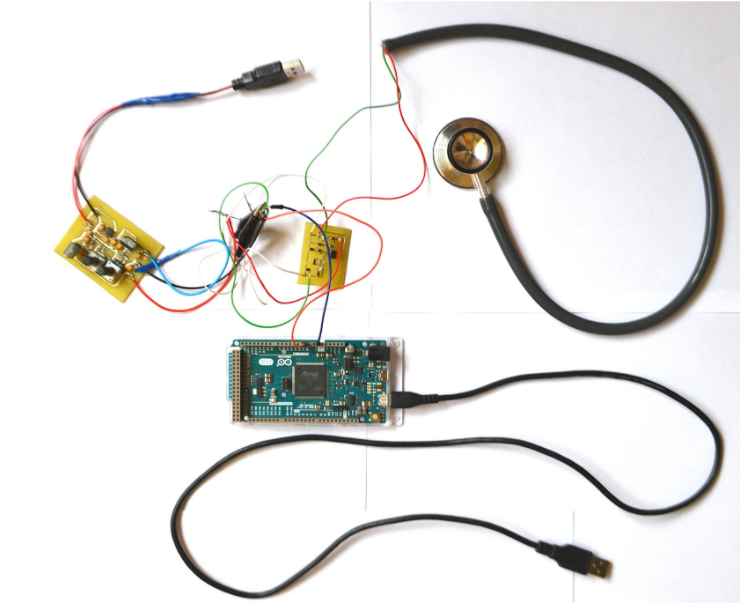
\includegraphics[width=14cm]{images/hardware.png}
% \caption{Собранный прототип}
% \end{figure}

\subsection{Описание микрофона}
В качестве микрофона был выбран SWEN MK-200. \\

\begin{table}[h]
\centering
\label{my-label}
\begin{tabular}{|l|l|}
\hline
Чувствительность, дБ           & -60 ± 3                    \\ \hline
Диапазон частот, Гц            & 50 – 16 000                \\ \hline
Размер микрофонного модуля, мм & 9×7                        \\ \hline
Тип разъема                    & мини-джек Ø 3,5 мм (3 pin) \\ \hline
Длина кабеля, м                & 1,8                        \\ \hline
Вес, г                         & 63                         \\ \hline
\end{tabular}
\caption{Технические характеристики SWEN MK-200}
\end{table}

Микрофон был вынут из стандартного корпуса, чтобы лучше соединиться с трубкой, ведущей к мембране.

\subsection{Описание усилителя}
Усилитель для микрофона был создан самостоятельно в рамках данной работы.

Была выбрана следующая схема усилителя:

\begin{figure}[H]
\centering
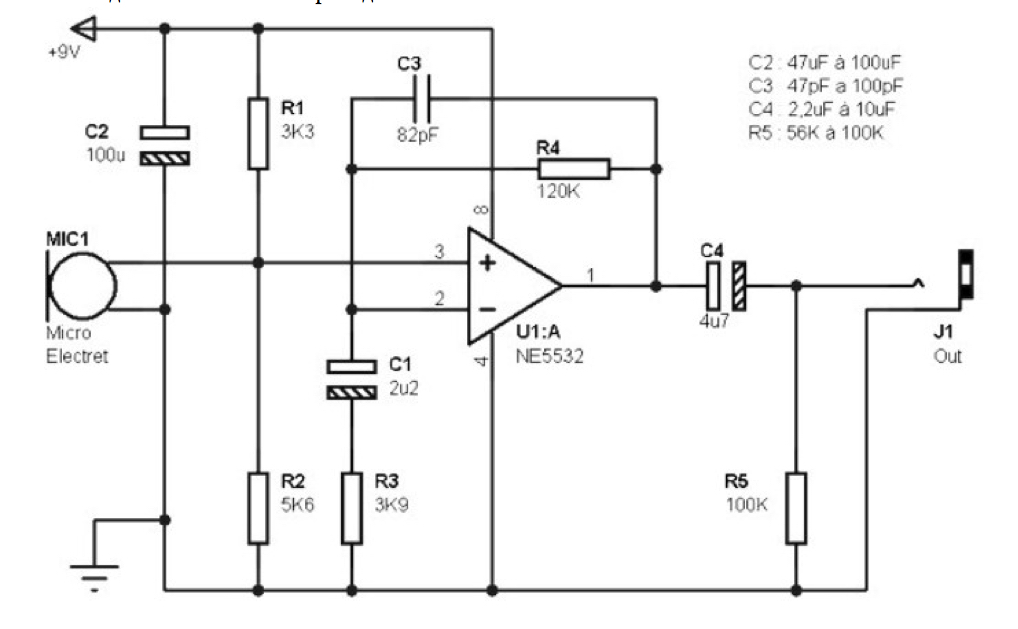
\includegraphics[width=14cm]{images/circuit.jpg}
\caption{Схема усилителя сигнала}
\end{figure}

В качестве операционного усилителя был выбран \textbf{MCP6022} от производителя Microchip. Это усилитель типа Rail-to-Rail SO-8.

SOIC или просто SO (small-outline-integrated-circuit), а также SOP (Small-Outline Package) корпус микросхем, предназначенный для поверхностного монтажа, занимающий на печатной плате на 30-50\% меньше площади чем аналогичный корпус DIP, а также имеющий на 50-70\% меньшую толщину. Обычно в обозначении также указывается число выводов.

В данный усилитель встроены High-Pass и Low-Pass фильтры. High-Pass фильтрует частоты сигнала меньше 1Гц. Low-Pass фильтрует частоты выше 100кГц. Меняя конденсатор С3, можно менять частоту среза LowPass фильтра. Усиление схемы зависит от резисторов R3 и R4. На текущий момент усиление составляет порядка 100.

Ниже приводятся параметры операционного усилителя.

\begin{table}[h]
\centering
\label{my-label}
\begin{tabular}{|l|l|}
\hline
Полоса частот                  & 10МГц                      \\ \hline
Уровень шума                   & 8.7 нВ/√Гц                 \\ \hline
Количество каналов             & 2                          \\ \hline
Напряжение питания             & 2.5В --- 5.5В              \\ \hline
Напряжение смещения            & $\pm500\mu V $             \\ \hline
Гармонические искажения        & 0.00053\%                  \\ \hline
Температурный диапазон         & -40°C --- +85°C            \\ \hline
Тип корпуса                    & SO-8                       \\ \hline
\end{tabular}
\caption{Технические характеристики операционного усилителя MCP6022}
\end{table}

\begin{figure}[H]
\centering
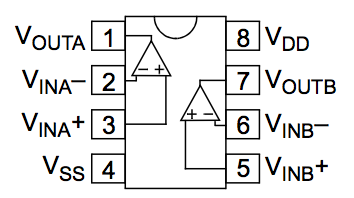
\includegraphics[width=12cm]{images/op-amp.png}
\caption{Распиновка операционного усилителя}
\end{figure}

\begin{figure}[H]
\begin{subfigure}{0.5\textwidth}
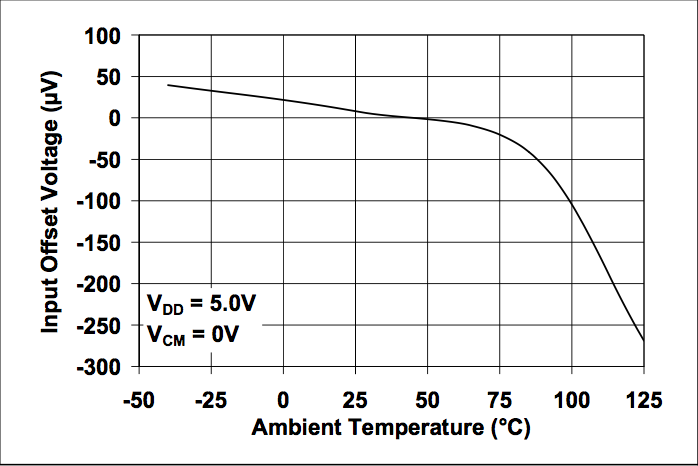
\includegraphics[width=0.9\linewidth, height=5cm]{images/op-amp-plot1.png} 
\caption{Напряжение смещения --- Температура}
% \label{fig:subim1}
\end{subfigure}
\begin{subfigure}{0.5\textwidth}
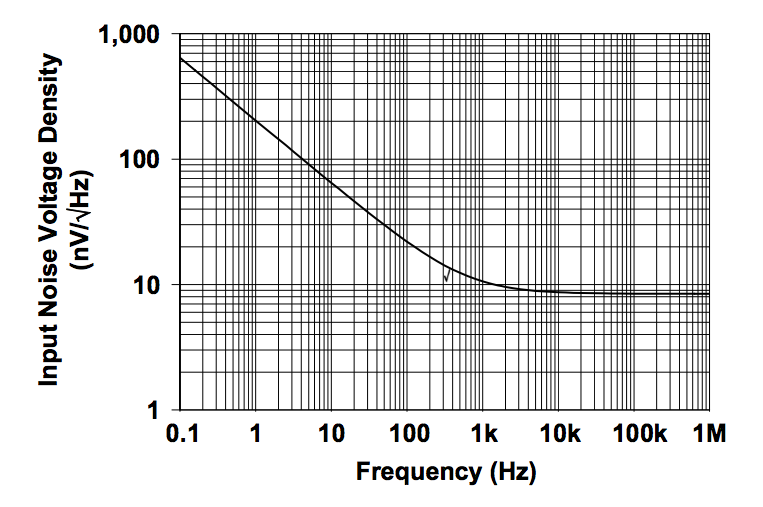
\includegraphics[width=0.9\linewidth, height=5cm]{images/op-amp-plot2.png}
\caption{Шум --- Частота}
% \label{fig:subim2}
\end{subfigure}

\vspace{10mm} % vertical space
 
\begin{subfigure}{0.5\textwidth}
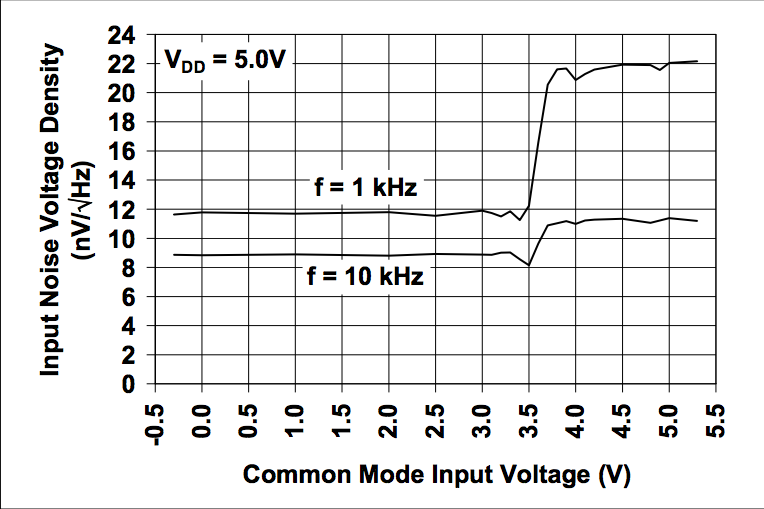
\includegraphics[width=0.9\linewidth, height=5cm]{images/op-amp-plot3.png} 
\caption{Шум - Напряжение смещения}
% \label{fig:subim1}
\end{subfigure}
\begin{subfigure}{0.5\textwidth}
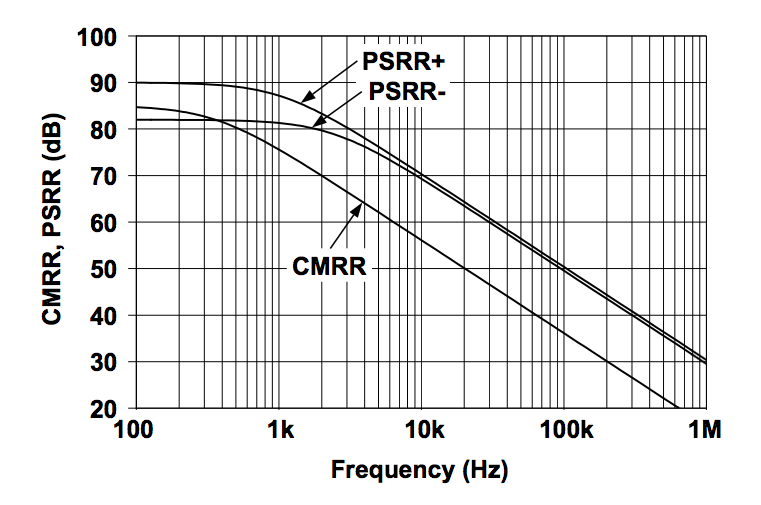
\includegraphics[width=0.9\linewidth, height=5cm]{images/op-amp-plot4.png}
\caption{CMRR --- Частота}
% \label{fig:subim2}
\end{subfigure}

\vspace{10mm} %vertical space

\begin{subfigure}{0.5\textwidth}
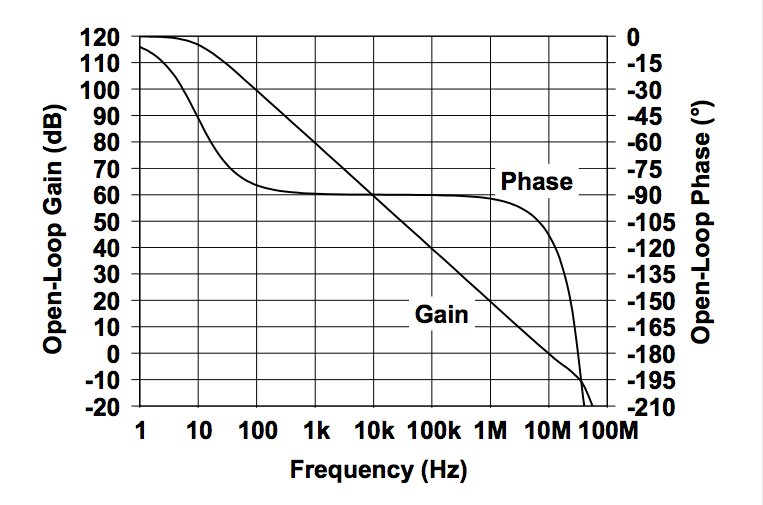
\includegraphics[width=0.9\linewidth, height=5cm]{images/op-amp-plot5.png} 
\caption{Коэффициент усиления - Частота}
% \label{fig:subim1}
\end{subfigure}
\begin{subfigure}{0.5\textwidth}
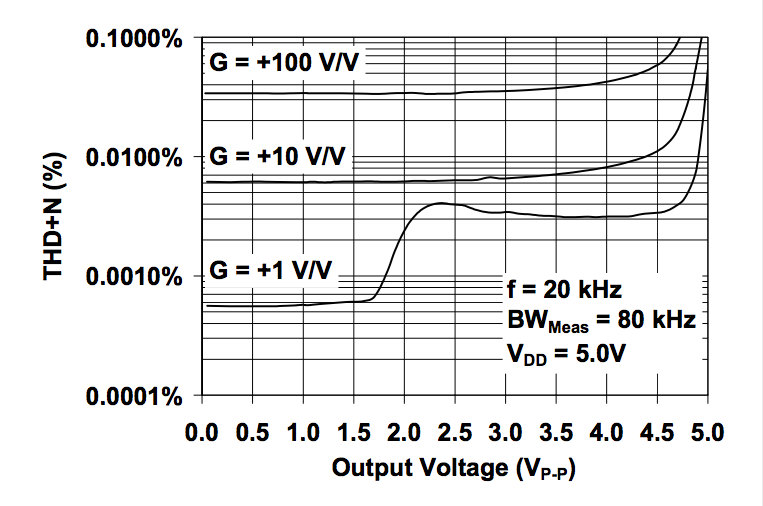
\includegraphics[width=0.9\linewidth, height=5cm]{images/op-amp-plot6.png}
\caption{\small{Гармонические искажения --- Вых. напряжение (f=20кГц)}}
% \label{fig:subim2}
\end{subfigure}

\caption{Параметры операционного усилителя}
\label{fig:image2}
\end{figure}

Разработка платы усилителя велась в программе Sprint Layout. Ниже представлен скриншот макета платы из этой программы.

\begin{figure}[H]
\centering
% \includegraphics[width=14cm]{sprint-layout-circuit.png}
\includegraphics[width=\textwidth]{images/sprint-layout-circuit.png}
\caption{Схема печатной платы усилителя}
\end{figure}

Печатная плата изготавливалась при помощи печати на лазерном принтере методом травления текстолита. 
\subsection{АЦП}
В качестве аналого цифрового преобразователя был выбран ЛА-н10-12USB от компании ЗАО "Руднев-Шиляев". Также стетоскоп тестировался на АЦП E-140 от компании LCard. 

Предназначение АЦП – преобразование непрерывных (аналоговых) входных сигналов в цифровую форму для дальнейшей обработки с помощью компьютера.

\begin{table}[h]
\centering
\label{my-label}
\begin{tabular}{|l|l|}
                                                                      \hline
Число аналоговых входов            & 2                             \\ \hline
Минимальная частота дискретизации  & 1.25МГц                       \\ \hline
Максимальная частота дискретизации & 80МГц                         \\ \hline
Объем буффера памяти               & $2\times10^{19}=524288$       \\ \hline
Разрядность                        & 12бит (4096 значений)         \\ \hline
Входное сопротивление              & 50Ом                          \\ \hline
Разъем                             & BNC                           \\ \hline
Диапазоны входного напряжения      & $\pm2V;\pm1V;\pm0.4V;\pm0.2V$ \\ \hline
Защита по входному напряжению      & $\pm5V$                       \\ \hline
Дифференциальная нелинейность      & $\pm1.2$ МЗР                  \\ \hline
Интегральная нелинейность          & $\pm1.5$ МЗР                  \\ \hline
Ошибка сдвига                      & $\pm0.15\%$                   \\ \hline
Интерфейс                          & USB                           \\ \hline
Потребляемая мощность              & 12В, 0.7А                     \\ \hline
Масса                              & 400г                          \\ \hline
\end{tabular}
\caption{Технические характеристики АЦП ЛА-н10-12USB}
\end{table}

\textbf{Интегральная нелинейность} - отклонение по вертикальной оси точек реальной характеристики от идеальной характеристики преобразования, делящих пополам расстояние по оси абцисс между средними значениями пороговых уровней характеристики преобразования. Измеряется в процентах или  МЗР.

\textbf{Дифференциальная нелинейность} - отклонение разности двух аналоговых сигналов от значения, соответствующего единице МЗР.

Данный АЦП работает в режиме старт-стоп. Другими словами он периодически производит запуск, сбор данных(в буффер) и остановку. Это один полный цикл сбора данных. При этом полезное время - это сбор данных, а старт и стоп - бесполезное.

Время, за которое АЦП совершает полный цикл сбора данных и соотношение полезного и бесполезного времени отличается в зависимости от частоты дискретизации и размера буффера. Были произведены замеры времени для различных значений частоты дискретизации и размера буффера и были составлены следующие таблицы.

Во всех таблицах X: размер буффера, Y: частота дискр.

\begin{figure}[H]
\centering
% \includegraphics[width=14cm]{sprint-layout-circuit.png}
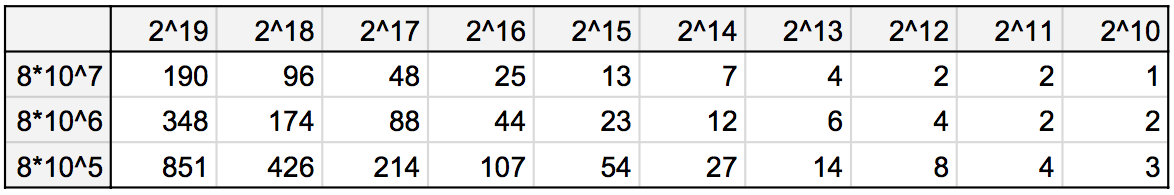
\includegraphics[width=\textwidth]{images/cycle-time.png}
\caption{Время на полный цикл (мс)}
\end{figure}

\begin{figure}[H]
\centering
% \includegraphics[width=14cm]{sprint-layout-circuit.png}
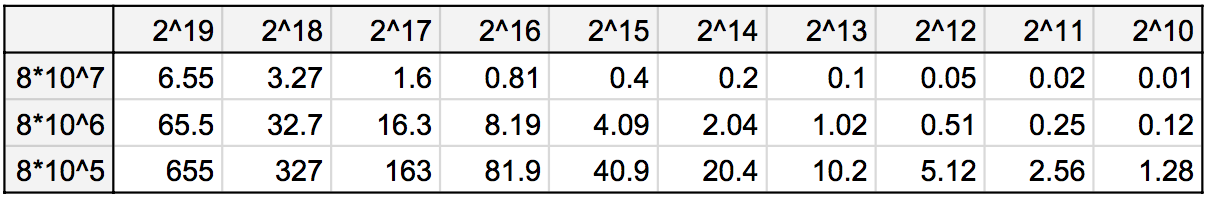
\includegraphics[width=\textwidth]{images/good-time.png}
\caption{Полезное время (мс)}
\end{figure}

\begin{figure}[H]
\centering
% \includegraphics[width=14cm]{sprint-layout-circuit.png}
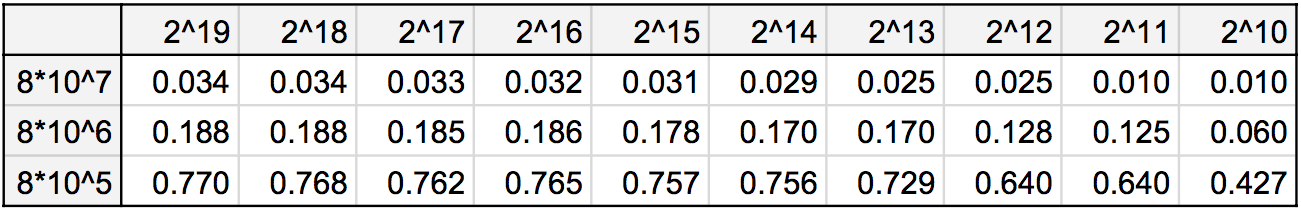
\includegraphics[width=\textwidth]{images/bad-div-by-good.png}
\caption{Отношение полезного времени к полному}
\end{figure}

\end{document}
